\subsection{Σχεδιαστικές αποφάσεις}

\subsubsection{Η αρχική ιδέα}

Ο στόχος του παιχνιδιού είναι να βοηθήσει νέους να εξοικειωθούν με τον τρόπο σκέψης που χρειάζεται ένας αλγόριθμος. Καθώς υπάρχουν αλγόριθμοι για διάφορες χρήσεις, επιλέχθηκε το παιχνίδι να εστιαστεί σε αλγόριθμους ταξινόμησης, διότι ποικίλουν σε πολυπλοκότητα, αλλά την ίδια στιγμή λύνουν ένα απλό καθημερινό πρόβλημα, την ταξινόμηση τιμών.

Ένα παιχνίδι, από τη φύση του, μπορεί να υπάρχει σε οποιαδήποτε μορφή και να είναι όσο πιο απλό, ή όσο πιο πολύπλοκο μπορεί κανείς να φανταστεί. Το γεγονός αυτό, καθιστά την ανάπτυξη ενός παιχνιδιού απολαυστική, καθώς το όριο είναι η φαντασία, αλλά συγχρόνως και δύσκολη, αφού δεν είναι εύκολο να σχεδιαστεί κάποια ροή παιχνιδιού με την οποία να είναι όλοι ικανοποιημένοι. Αυτό το εμπόδιο εμφανίστηκε και σε αυτό το παιχνίδι, καθώς το τελικό αποτέλεσμα προέκυψε ύστερα από πολλές διαφορετικές μορφές.

Η πρώτη ιδέα ήταν μία προσπάθεια να αναπαρασταθεί η μνήμη ενός υπολογιστή. Ακολουθώντας την δομή μιας μνήμης δεδομένων η οποία έχει διευθύνσεις, η ιδέα ήταν να υπάρχουν αριθμοί σε ακανονιστη σειρά, τοποθετημένοι μέσα σε σπίτια (κελιά μνήμης) με διευθύνσεις στην άκρη ενός δρόμου. Ο παίκτης θα έπρεπε, περπατώντας το δρόμο, να εισέλθει στα σπίτια και να μεταφέρει τις τιμές από το ένα σπίτι στο άλλο με βάση κάποιον προεπιλεγμένο αλγόριθμο ταξινόμησης. Αυτή η ιδέα τελικά εγκαταλείφθηκε διότι, ο χρόνος που ο παίκτης έπρεπε να ξοδέψει για να μεταβεί από το ένα σπίτι στο επόμενο ήταν πολύ μεγάλος, κάτι το οποίο είναι κουραστικό για ένα παίκτη.

Η δεύτερη ιδέα βασίστηκε πάνω στη πραγματική συμπεριφορά ενός υπολογιστή και τις μεταφορές που συμβαίνουν από και προς μια μνήμη. Ο παίκτης θα βρισκόταν σε ένα κόσμο “μέσα” σε έναν υπολογιστή, και θα αναλάμβανε να μεταφέρει τις τιμές από ένα κελί μνήμης στον επεξεργαστή και πίσω. Θα ήταν δηλαδή ένα ηλεκτρικό σήμα που ακολουθούσε τις οδηγίες του επεξεργαστή. Προφανώς η διαδικασία ήταν αρκετά απλοποιημένη από την πραγματική, αλλά ακόμη και με τις απλοποιησεις κρίθηκε πως το παιχνίδι θα ήταν πολύ περίπλοκο, ειδικά για νέους που δεν γνωριζουν βασικές πληροφορίες για τη λειτουργία ενός υπολογιστή.

Καθώς καμία από τις παραπάνω δεν ήταν αρκετά ικανοποιητική, μετά από επανασχεδιασμό, το παιχνίδι κατέληξε να έχει την τελική του μορφή.

% ========================================

\subsubsection{Το παιχνίδι σήμερα}

Μετά τον επανασχεδιασμό αποφασίστηκε η βασική ροή του παιχνιδιού να απλοποιηθεί αρκετα και να υπάρχουν άλλα υποστηρικτικά συστήματα να το κάνουν πιο ενδιαφέρον.

\textbf{Δημιουργία τιμών}

Η δημιουργία των κουτιών που περιέχουν τις τιμές συμβαίνει δυναμικά, με βάση ρυθμίσεις που υπάρχουν στη βάση δεδομένων. Σε αυτή έχει πρόσβαση ο εκπαιδευτικός και έχει τη δυνατότητα να ρυθμίσει τον αριθμό των κουτιών που δημιουργούνται, καθώς και τη μεγαλύτερη και μικρότερη τιμή που μπορούν να πάρουν. Οι ίδιες οι τιμές δημιουργούνται τυχαία με βάση αυτές τις παραμέτρους μέσα στο παιχνίδι όταν μπει ο παίκτης.

\textbf{Βασική ροή}

Αρχικά οι τιμές θα βρίσκονται μέσα σε κουτιά με τα οποία θα μπορεί ο παίκτης να αλληλεπιδράσει και να μετακινήσει τις τιμές. Ο στόχος είναι, ακολουθώντας έναν επιλεγμένο αλγόριθμο, να ταξινομήσει τις τιμές. Η λογική αυτή είναι παρόμοια με αυτή της αρχικής ιδέας, αλλά με αρκετά πιο γρήγορο ρυθμό.

\begin{figure}[H]
    \centering
    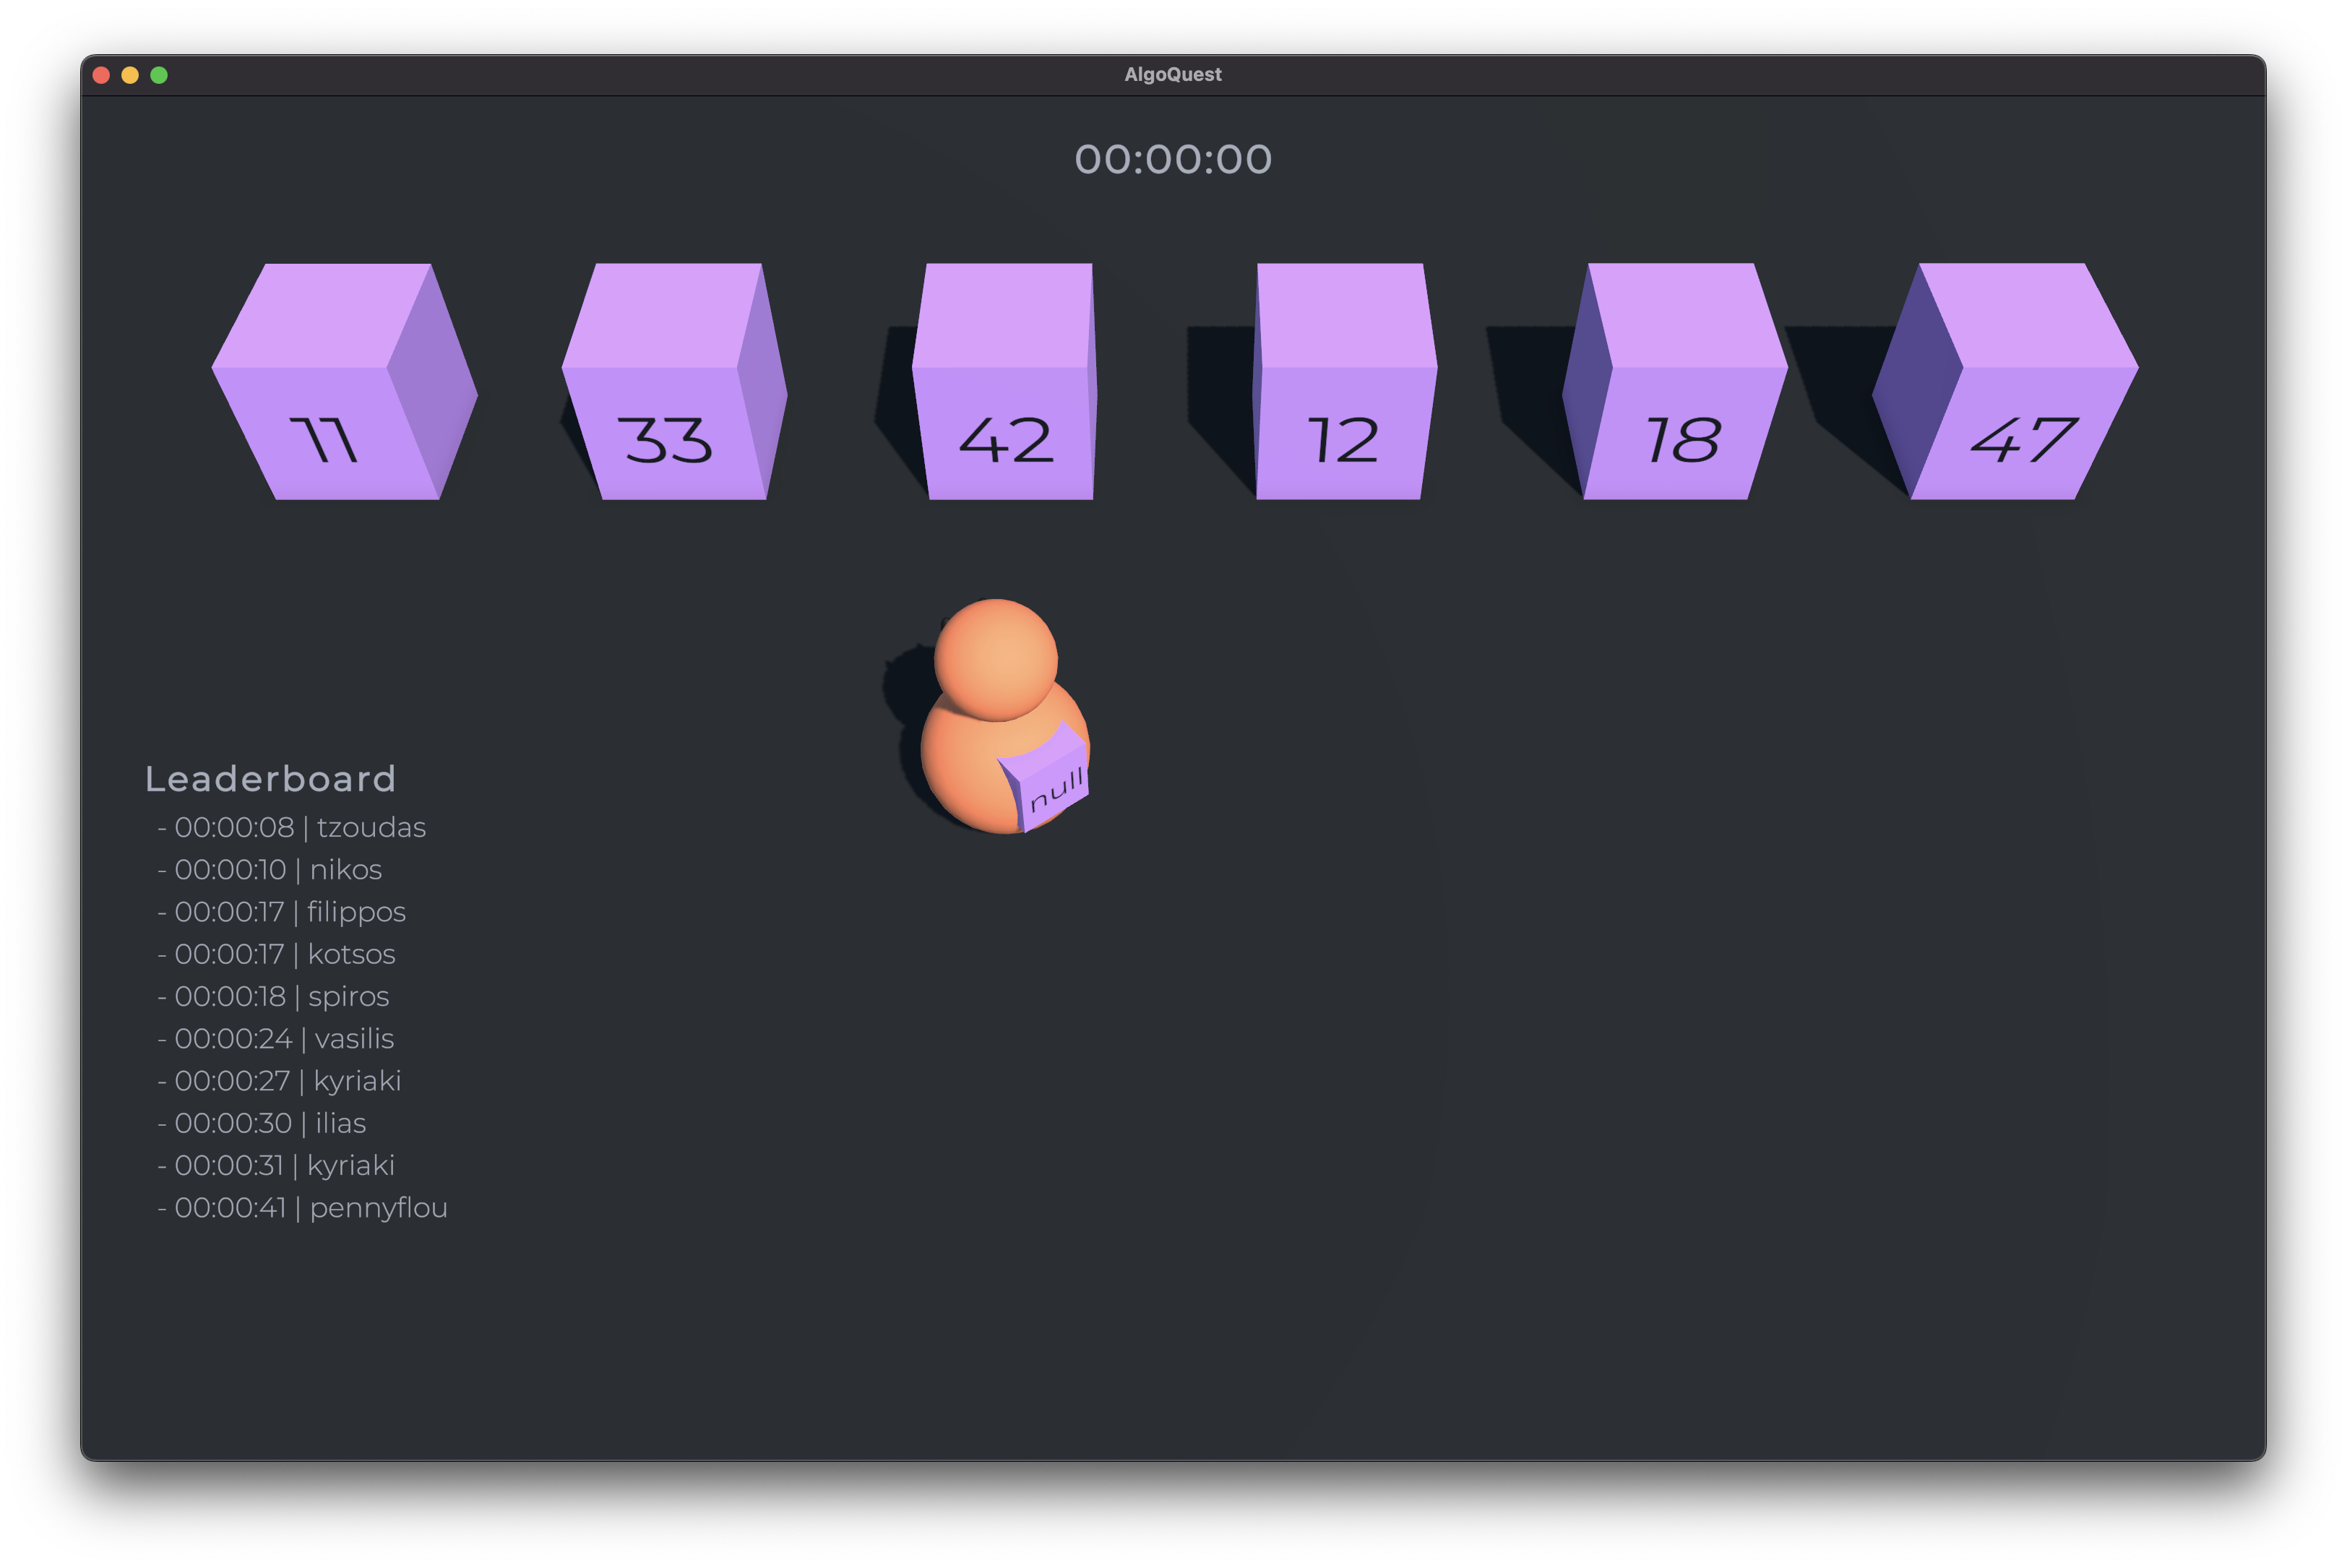
\includegraphics[width=0.8\linewidth]{sections/4/2/images/game_solo}
    \caption{Η οπτική του παίκτη στο παιχνίδι.}
    \label{fig:game_solo}
\end{figure}

Καθώς όμως αυτή η ροή δεν είναι αρκετή για να κινήσει το ενδιαφέρον του παίκτη, υπήρξε το ερώτημα για το ποιά μέθοδος μπορεί να χρησιμοποιηθεί, η οποία θα έκανε το παιχνίδι πιο ενδιαφέρον, χωρίς όμως αυξάνει την πολυπλοκότητα.

Η χρονομέτρηση μιας διαδικασίας ενάντια στο χρόνο υπάρχει για πάρα πολλά χρόνια και χρησιμοποιείται και στον αθλητισμό, αλλά και στα παιχνίδια, γνωστό ως \gls{time_trial}. Η ιδέα είναι απλή: ένας παίκτης προσπαθεί να εκτελέσει κάτι μέσα σε ένα παιχνίδι όσο πιο γρήγορα μπορεί με σκοπό να εξασφαλίσει τον καλύτερο χρόνο. Αυτό έχει ως αποτέλεσμα να προκαλέσει μία αίσθηση επείγοντος στον παίκτη καθώς μάχεται ενάντια σε άλλους παίκτες για τον καλύτερο χρόνο. Η χρήση ενός τέτοιου συστήματος για το παιχνίδι λοιπόν, θα έχει το επιθυμητό αποτέλεσμα. Η ροή που θα πρέπει ο παίκτης να ακολουθήσει για να ταξινομήσει τις τιμές δεν αλλάζει, αλλά την ίδια στιγμή θα προσπαθεί να έχει τον καλύτερο χρόνο, κάτι το οποίο θα τον βυθίσει στο παιχνίδι και θα τον βοηθήσει να κατανοήσει αυτό που κάνει αλλά και να απολαύσει τη διαδικασία.

\textbf{Αλγόριθμοι}

Τα βήματα τα οποία πρέπει να πάρει ένας παίκτης για να ταξινομήσει τις τιμές αλλάζουν ανάλογα με τον επιλεγμένο αλγόριθμο. Καθώς η υλοποίηση ενός νέου Scene για κάθε αλγόριθμο με τις σωστές κινήσεις και συγκεκριμένους αριθμούς δεν ήταν κάτι θεμιτό, λόγο του φόρτου που θα χρειαζόταν για κάθε διαφορετικό αλγόριθμό, επιλέχθηκε να υλοποιηθεί ένα σύστημα το οποίο θα λειτουργούσε για κάθε αλγόριθμο ταξινόμησης. Αυτό το σύστημα είναι ένα Unity Script από το οποίο μπορεί ο χρήστης να επιλέξει έναν αλγόριθμο και το Script θα υπολογίσει τα σωστά βήματα για αυτόν.

\begin{figure}[H]
    \centering
    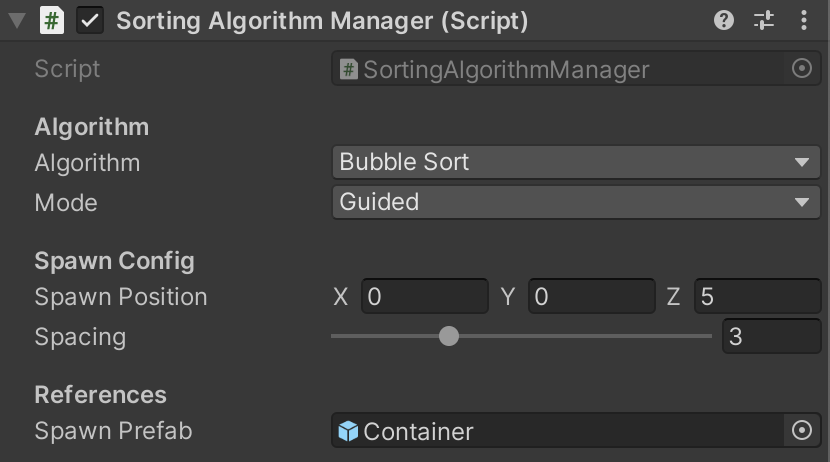
\includegraphics[width=0.6\linewidth]{sections/4/2/images/unity_editor_sorting_algorithm_manager}
    \caption{Script ρυθμίσεων για τον αλγόριθμο του παιχνιδιού}
    \label{fig:unity_editor_sorting_algorithm_manager}
\end{figure}

Tο Script αυτό δουλεύει ως εξής:
\begin{itemize}
    \item Διαβάζει τις ρυθμίσεις που έχει θέσει ο εκπαιδευτικός για τον αλγόριθμο μέσω του διαχειριστικού (Κεφάλαιο \ref{sssec:admin_dashboard}).
    \item Υπολογίζει τη θέση που πρέπει να τοποθετηθούν τα κουτιά τιμών ανάλογα με τον αριθμό τιμών.
    \item Δημιουργεί τις τιμές τυχαία, λαμβάνοντας υπόψη τα άνω και κάτω όρια που έχει θέσει ο εκπαιδευτικός.
    \item Εκτελεί τον επιλεγμένο αλγόριθμο για τις δημιουργημένες τιμές και αποθηκεύει τα ζευγάρια αλλαγών τιμών που χρειάζεται για να είναι επιτυχής η διαδικασία.
    \item Δημιουργεί τα κουτιά με τις αρχικές τιμές.
\end{itemize}

Το ίδιο Script είναι αυτό το οποίο παρακολουθεί τις κινήσεις του παίκτη και τις αλλαγές που εκτελεί, και κρίνει εάν έκανε μία σωστή ή μία λάθος κίνηση.

\begin{figure}[H]
    \centering
    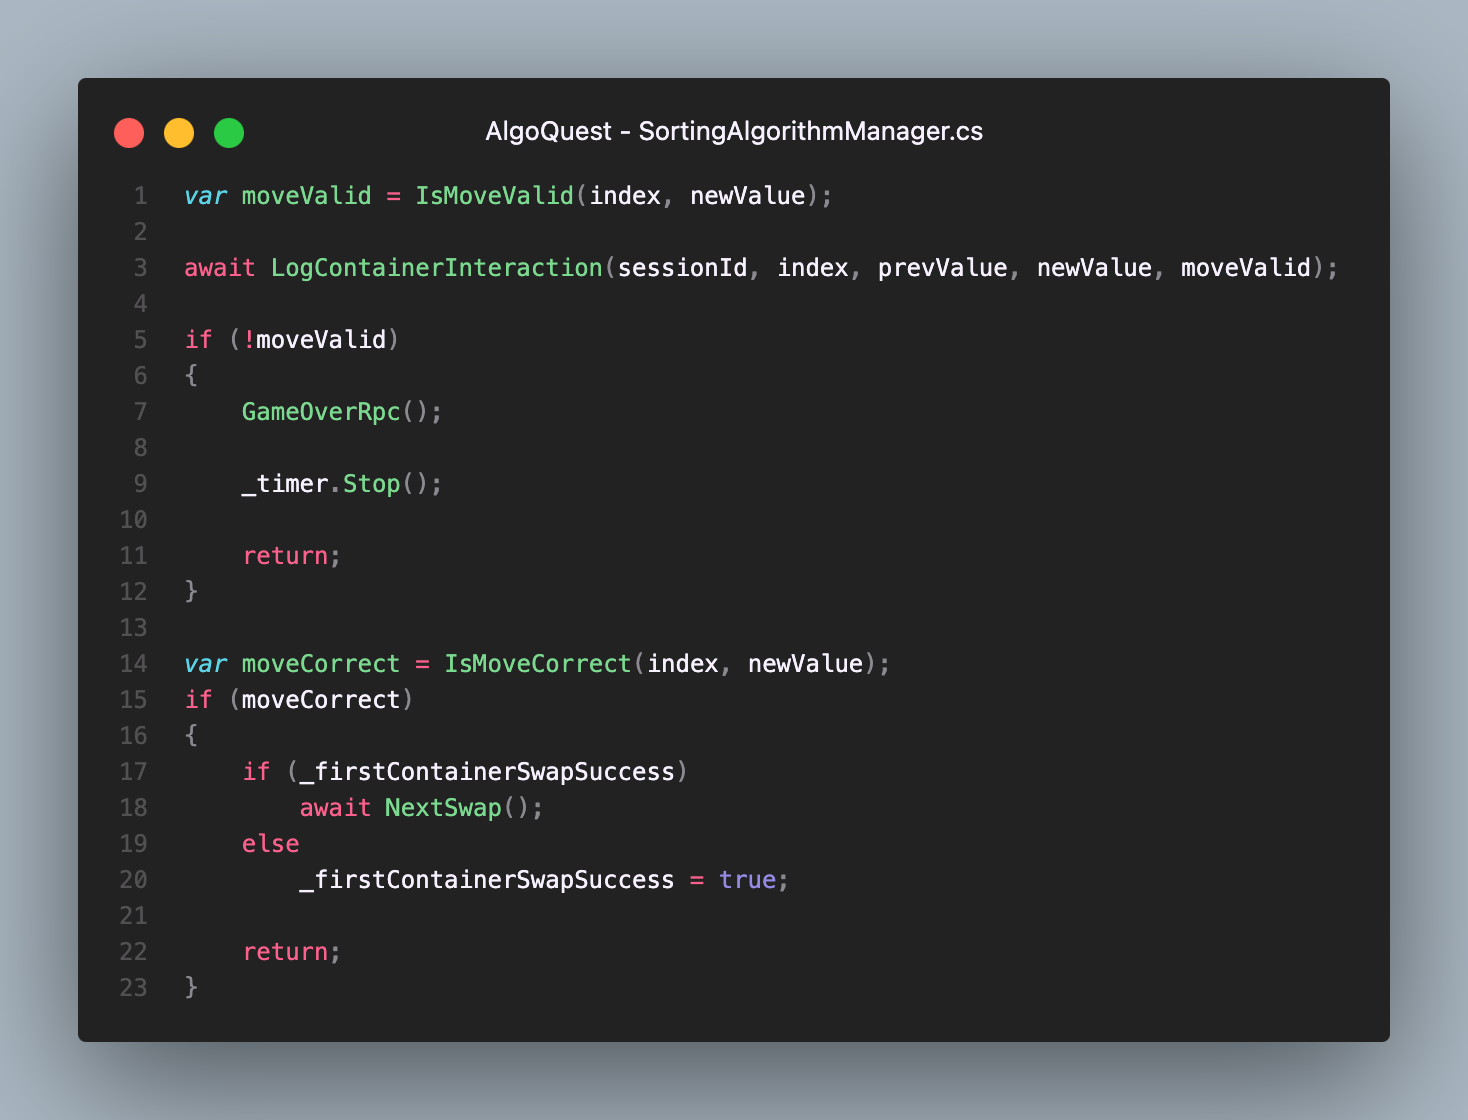
\includegraphics[width=0.8\linewidth]{sections/4/2/images/unity_code_sorting_algorithm_manager_move_valid}
    \caption{Απόσπασμα κώδικα για τον έλεγχο της ορθότητας της κίνησης του παίκτη}
    \label{fig:unity_code_sorting_algorithm_manager_move_valid}
\end{figure}

Η διαδικασία εκτέλεσης του αλγορίθμου, για κάθε επιλεγμένο αλγόριθμο προσφέρει το προνόμιο πως για να προστεθεί ένας νέος αλγόριθμος αρκεί κάποιος να υλοποιήσει τον πραγματικό αλγόριθμο ο οποίος απλώς θα ταξινομεί τιμές. Η υπόλοιπη διαδικασία είναι αυτόνομη και απλώς περιμένει μία λίστα από ζευγάρια αλλαγών τιμών (θέσεις και τιμές), όπως φαίνεται στην Εικόνα \ref{fig:unity_code_bubble_sort}.

\begin{figure}[H]
    \centering
    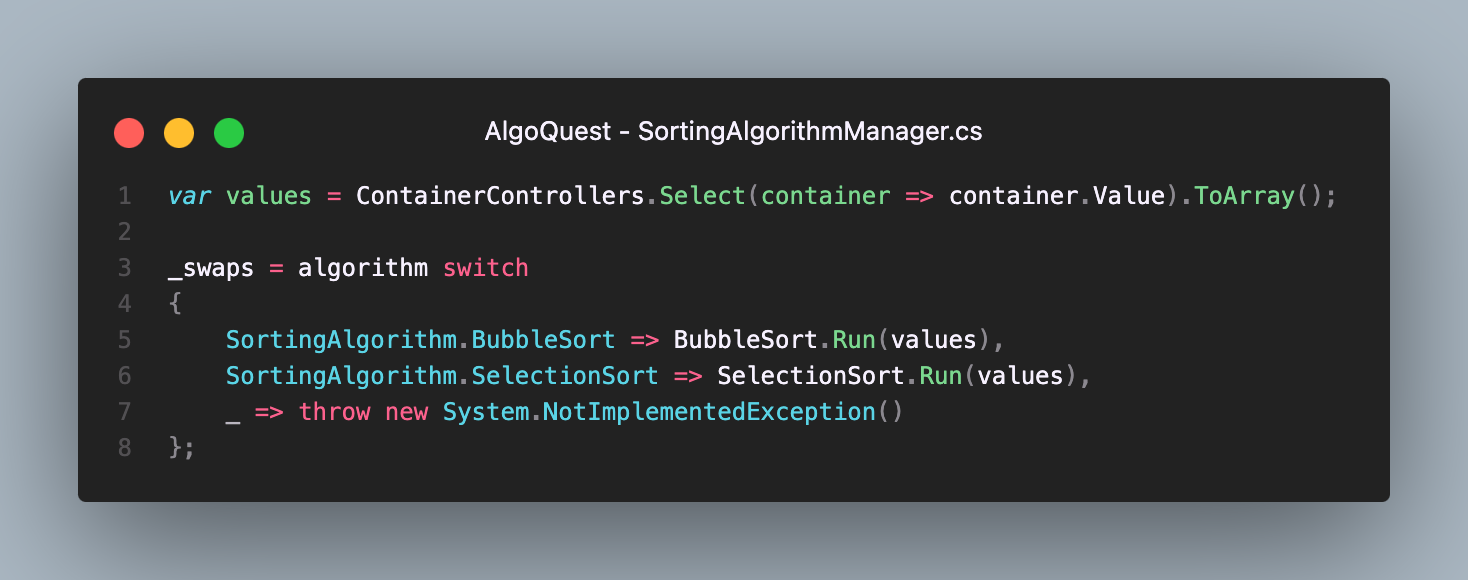
\includegraphics[width=0.8\linewidth]{sections/4/2/images/unity_code_sorting_algorithm_manager_algorithm_selection}
    \caption{Απόσπασμα κώδικα για την επιλογή του αλγορίθμου}
    \label{fig:unity_code_sorting_algorithm_manager_algorithm_selection}
\end{figure}

\begin{figure}[H]
    \centering
    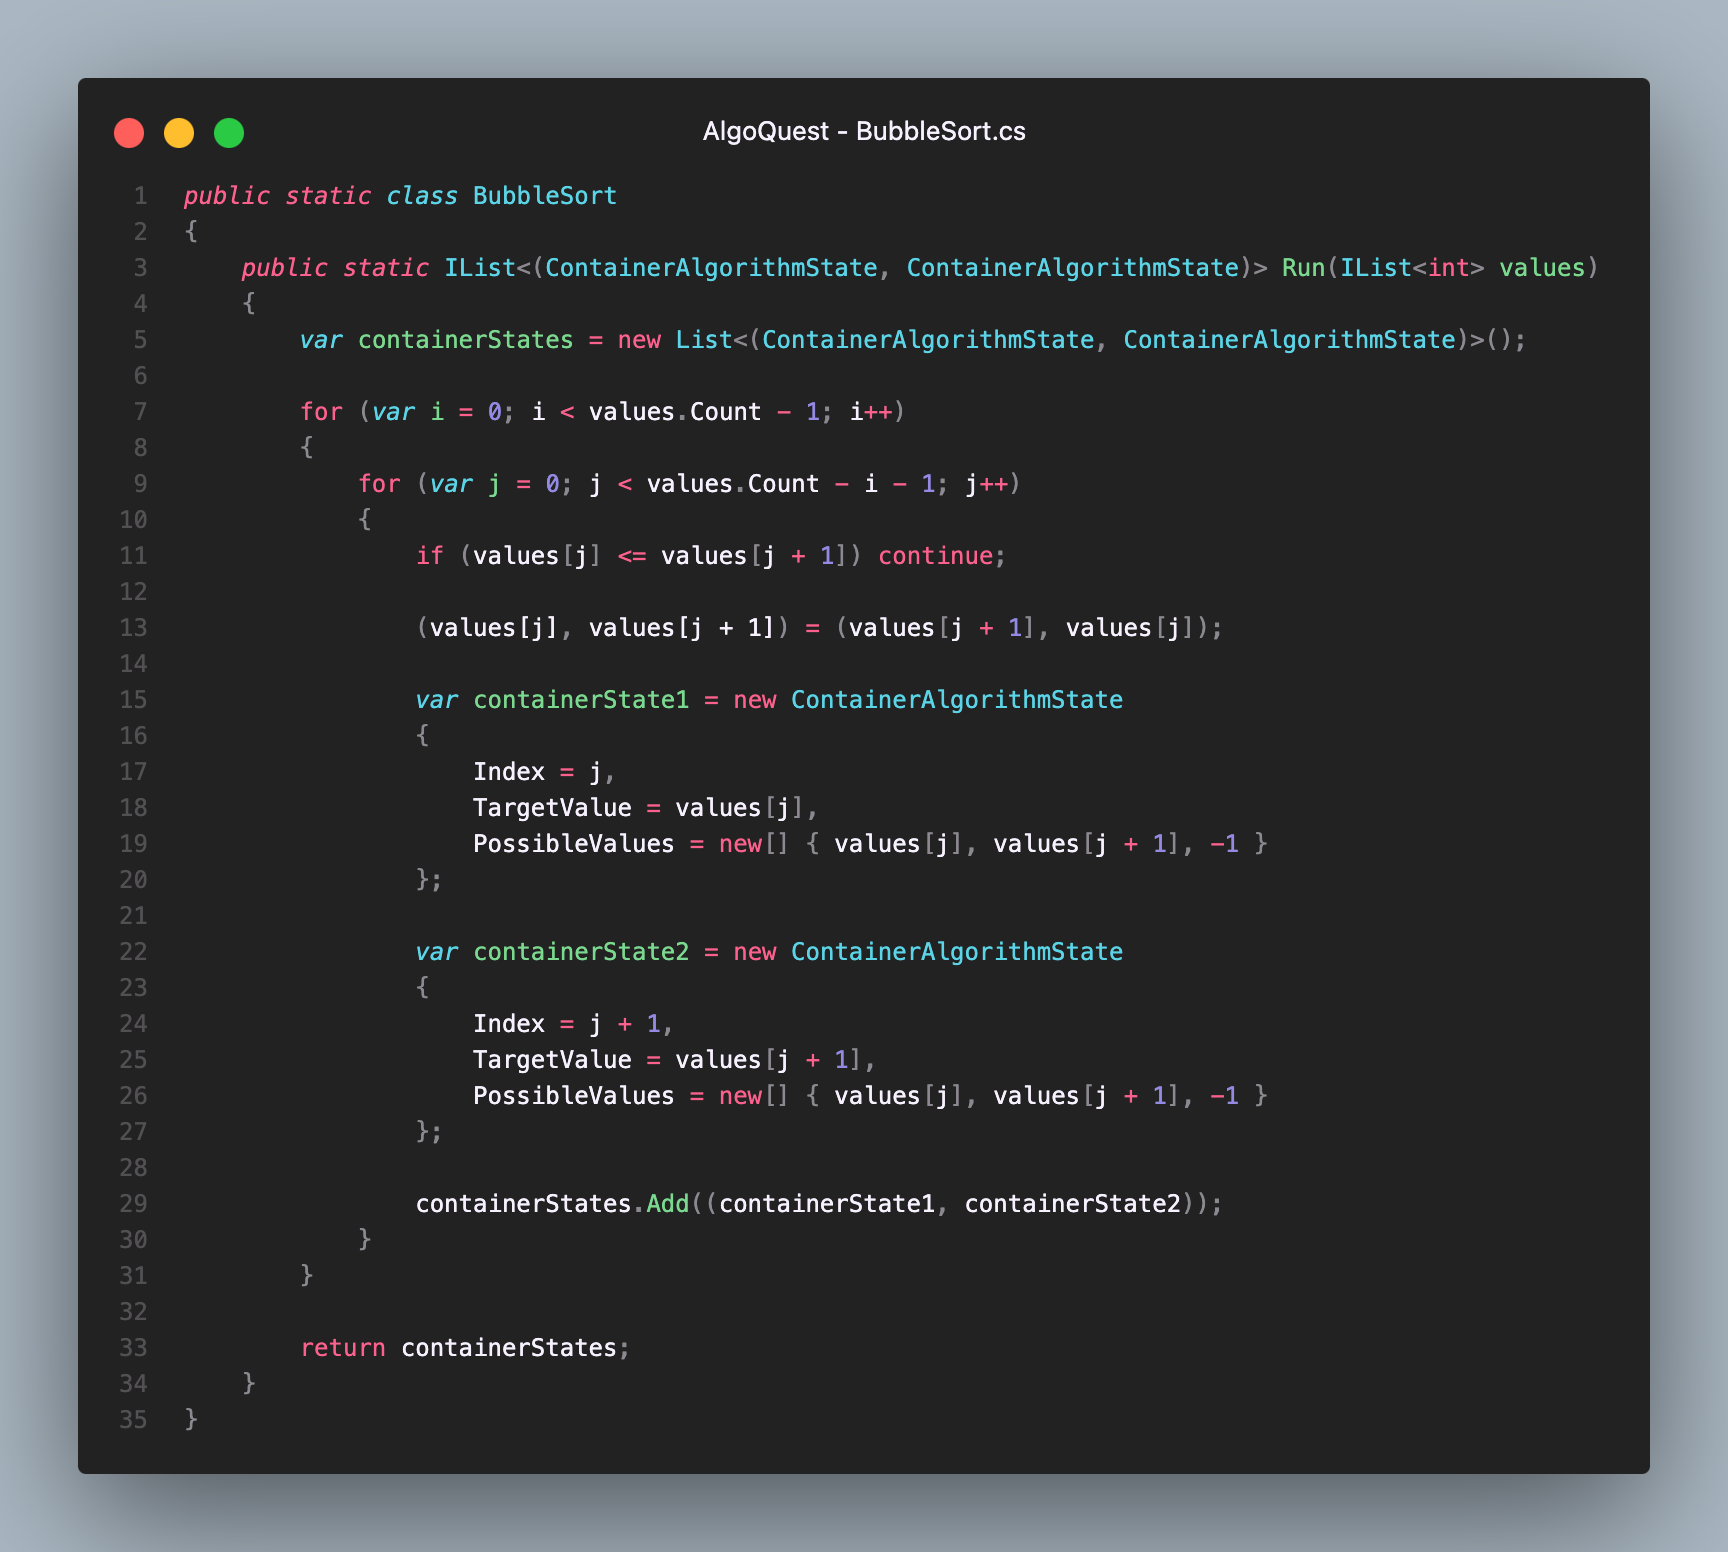
\includegraphics[width=0.8\linewidth]{sections/4/2/images/unity_code_bubble_sort}
    \caption{Κώδικας υπολογισμού των κινήσεων για τον αλγόριθμο Bubble Sort}
    \label{fig:unity_code_bubble_sort}
\end{figure}

\textbf{Επίπεδα δυσκολίας}

Η βασική ροή του παιχνιδιού έχει ένα πρόβλημα. Αυτό είναι πως δεν υπάρχουν πληροφορίες για το εάν μία κίνηση είναι σωστή ή λάθος, πέραν της αποτυχίας εάν γίνει λάθος κίνηση. Αυτό έχει ως αποτέλεσμα ένας νέος παίκτης να νιώθει χαμένος και όχι σίγουρος εάν αυτό που κάνει είναι σωστό. Το πρόβλημα αυτό μπορεί εύκολα να λυθεί με την βοήθεια και καθοδήγηση του εκπαιδευτικού, ο οποίος μπορεί να εξηγεί τι συμβαίνει σε κάθε βήμα του αλγορίθμου. Αυτό όμως δεν αποτελεί καλή λύση, διότι η επιθυμία ήταν να μπορεί κάποιος να παίξει το παιχνίδι μόνος του, εκτός των ορίων του διδακτικού τομέα.

Η λύση παρουσιάστηκε ως επίπεδα δυσκολίας. Αντί να αλλάξει η λογική και λειτουργία της βασικής ροής, η ιδέα ήταν να δημιουργηθεί και μία ακόμη ροή η οποία θα επικεντρώνεται στη βοήθεια και τη καθοδήγηση τον παικτών γύρω από τον επιλεγμένο αλγόριθμο. Σε αυτή τη ροή θα αφαιρεθεί το χρονόμετρο, δίνοντας έτσι στους παίκτες μεγαλύτερη άνεση με τις κινήσεις τους και αφαιρώντας το άγχος που προσφέρει. Συγχρόνως τα κουτιά που περιέχουν τις τιμές θα επιτρέπουν μονάχα τη μετακίνηση των σωστών τιμών. Αυτό δεν αφαιρεί πλήρως την ανάγκη για προαπαιτούμενη γνώση των αλγορίθμων, αλλά τη μειώνει δραστικά.

\begin{figure}[H]
    \centering
    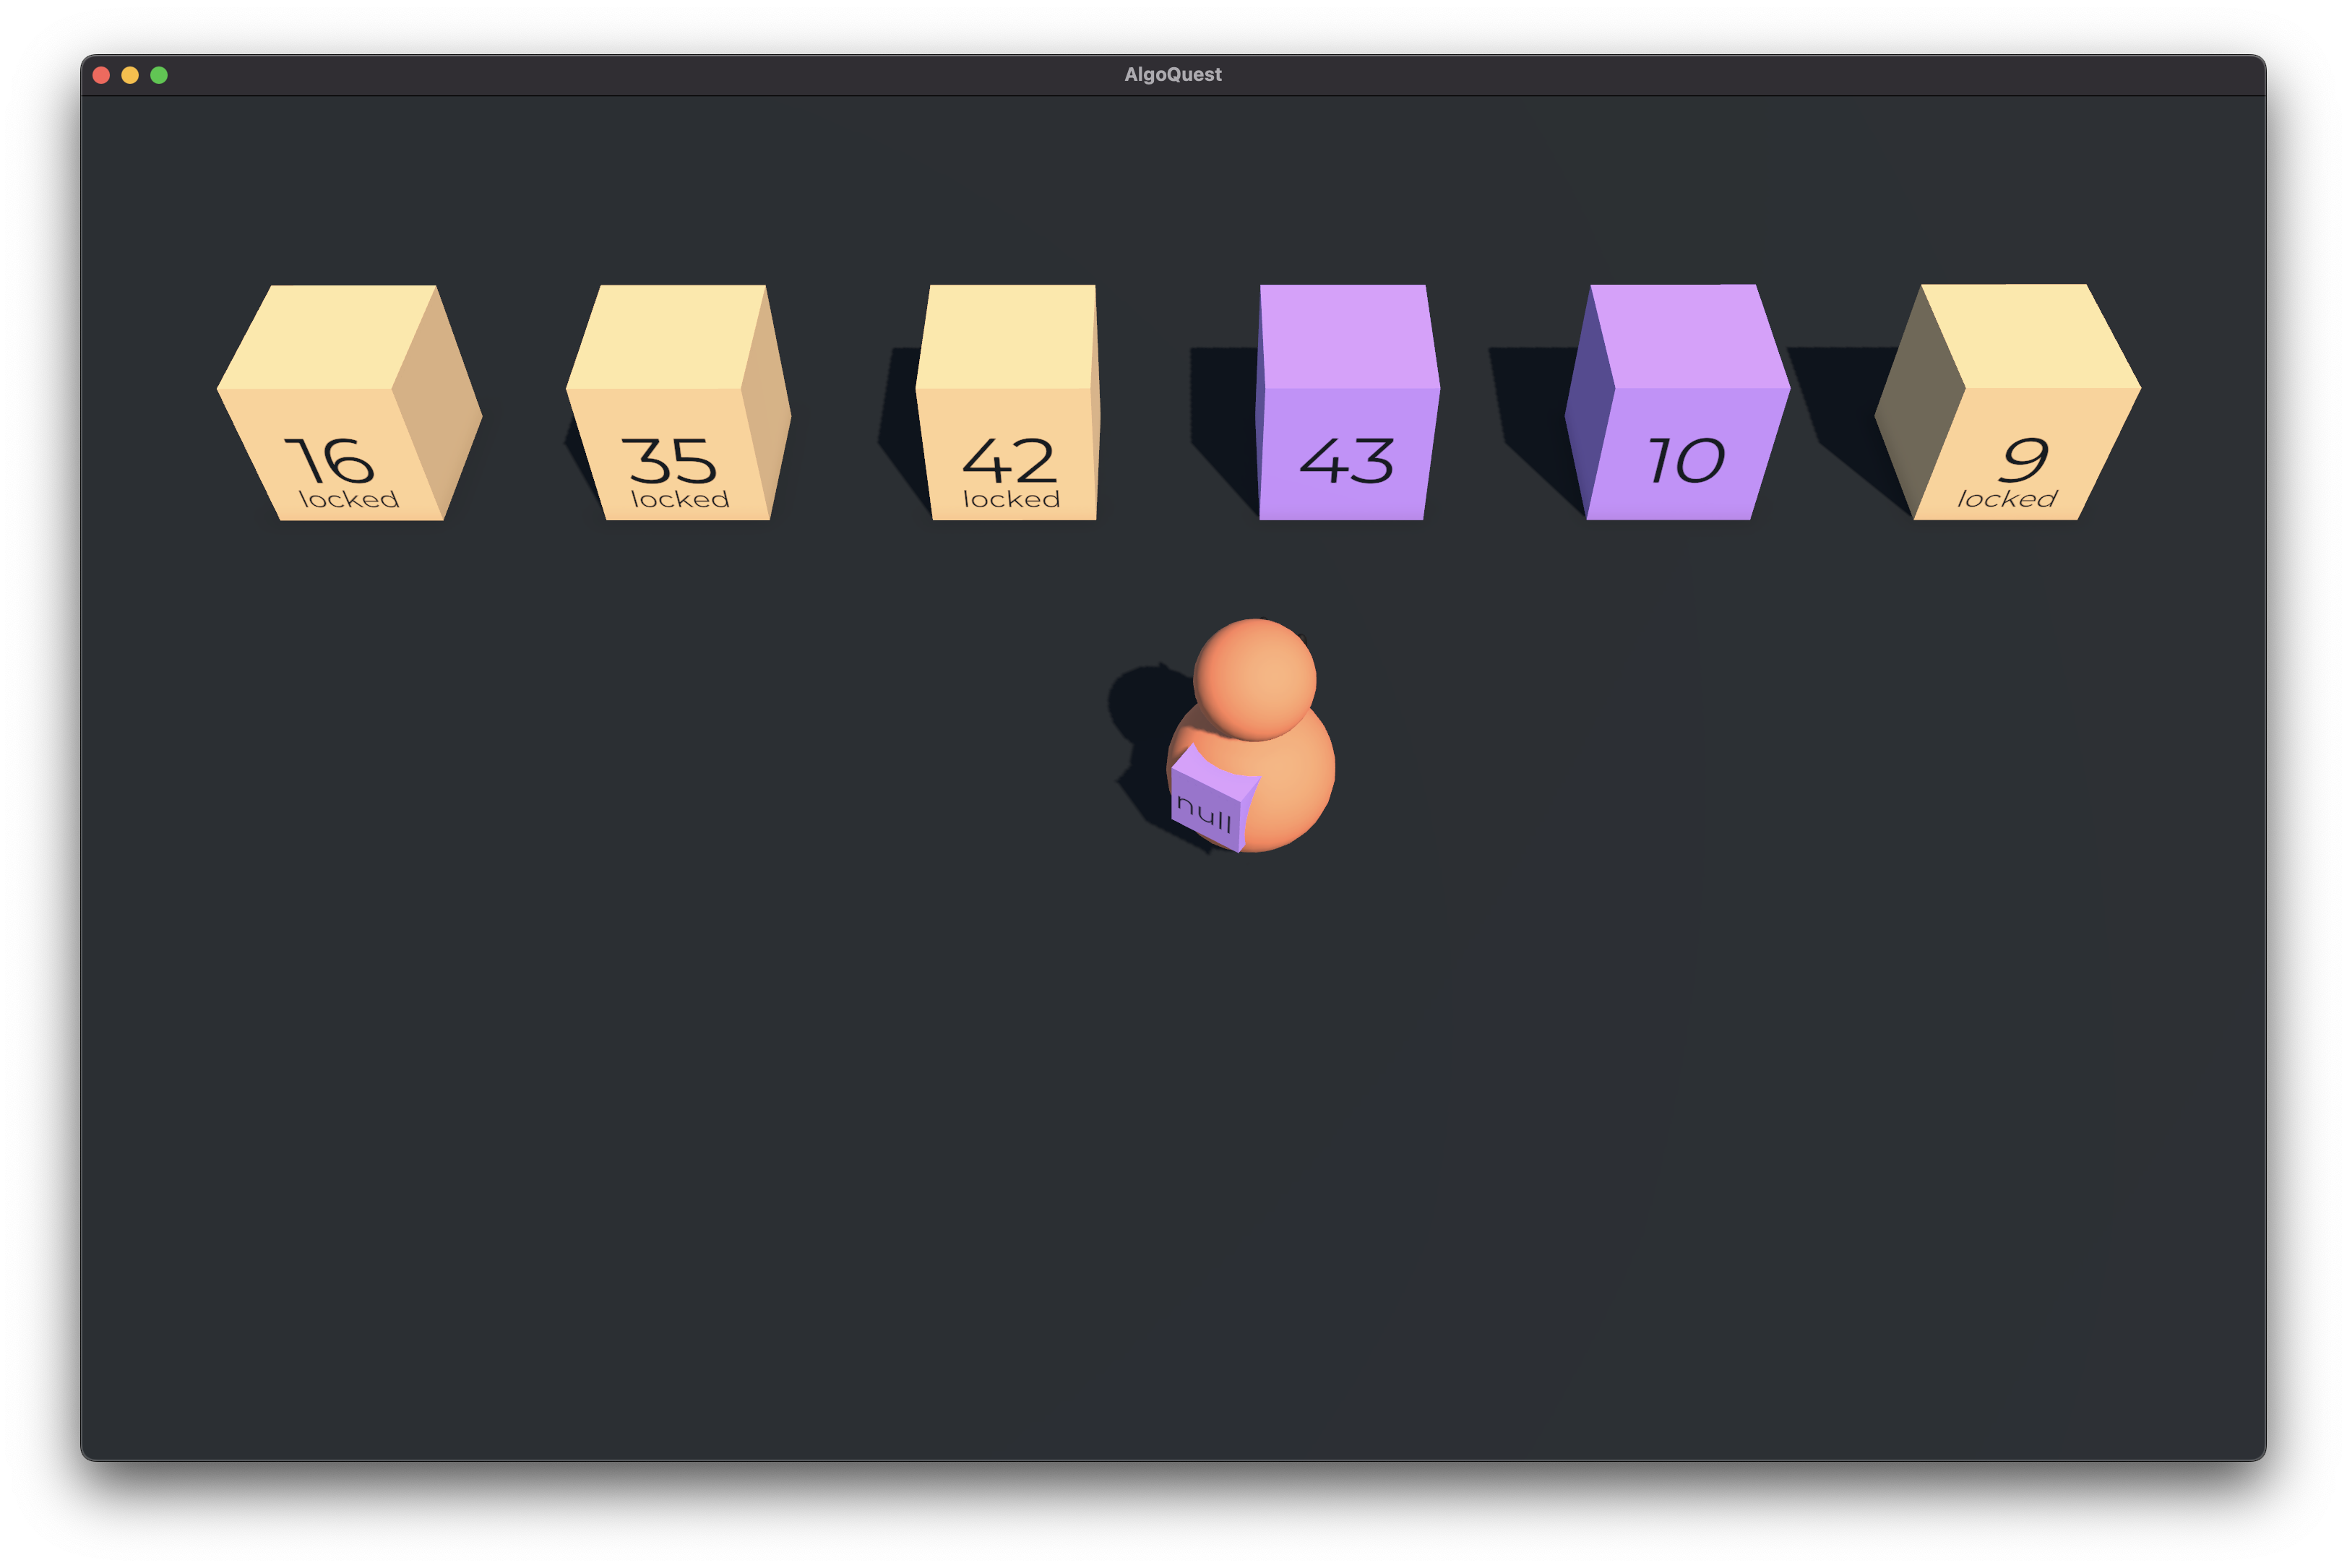
\includegraphics[width=0.8\linewidth]{sections/4/2/images/game_guided_mode}
    \caption{Το παιχνίδι σε καθοδηγούμενη λειτουργία}
    \label{fig:game_guided_mode}
\end{figure}
